\begin{abstract}
    Understanding human security and social equity issues within human systems requires large-scale models of population dynamics that simulate high-fidelity representations of individuals and access to essential activities (work/school, social, errands, health). Likeness is a Python toolkit that provides these capabilities for Oak Ridge National Laboratory's (ORNL) UrbanPop spatial microsimulation project. In step with the initial development phase for Likeness (2021 - 2022), we built out several foundational examples of work/school and health service access. In this paper, we describe expansion and scaling of Likeness capabilities to metropolitan areas in the United States. We then provide an integrated demonstration of our methods based on a case study of Leon County, FL and perform validation exercises on 1) neighborhood demographic composition and 2) visits by demographic cohorts (gender/age) obtained from point of interest (POI) footfall data for essential services (grocery stores). Taking into account lessons learned from our case study, we scope improvements to our model as well as provide a roadmap of the anticipated Likeness development cycle into 2023 - 2024.
\end{abstract}

\subsection{Introduction}\label{introduction}

Agent-based models (ABMs) of population dynamics are essential for understanding human security and social equity issues within human systems \cite{germann2022assessing, ozik2021population, urbanpop-AG-2023}. Such models often rely upon \emph{synthetic populations} -- virtual representations of individuals plausibly residing within an area -- to assess how individual behaviors and interactions contribute to complex system-level behavior. Applications of ABMs for population dynamics range from urban planning (access to essential services like food and healthcare), public health (facility occupancy, social contact networks), and disaster preparedness (social vulnerability to environmental hazards, evacuation and critical infrastructure planning).

A current challenge for research in population dynamics is to more directly represent population heterogeneity \cite{BRaVE_DOE_2022}. Individuals exhibit a variety of patterns of life dictating their behavior and interactions \cite{pappalardo2015returners}, which are in turn influenced by social, demographic, and economic characteristics. Incorporating these factors into the design of synthetic populations contributes to more holistic models of how human systems operate.

To support enhanced ABMs of population dynamics, the UrbanPop spatial microsimulation framework developed by Oak Ridge National Laboratory (ORNL) generates high-fidelity synthetic populations on hundreds of attributes from the American Community Survey (ACS) and its Public-Use Microdata Sample (PUMS) and combines them with nighttime/daytime behavioral routines \cite{urbanpop-AG-2023}. Central to UrbanPop's capabilities is Likeness, a Python toolkit that combines population synthesis, spatial network modeling, and activity allocation \cite{likeness-scipy-paper-2022, likeness-scipy-poster-2022}. Foundational examples produced for Likeness have explored travel routing from home locations to anchor activities (e.g., work, school), POI occupancy characteristics \cite{likeness-scipy-paper-2022, likeness-scipy-poster-2022}, as well as routing incidental travel from anchor to non-anchor activities (e.g., social, errands, health) \cite{likeness_aag_2023}. This paper builds from these foundational examples to
discuss scaling our methods to larger areas of interest. Moreover, it examines the performance of our activity allocation model relative to real-world POI demographics from digital trace (anonymized mobile device) data on POI visitation.

\subsection{Expansion and Scaling of Likeness Capabilities}\label{section:likeness-expansion-scaling}

\begin{figure*}[htbp]
\centering
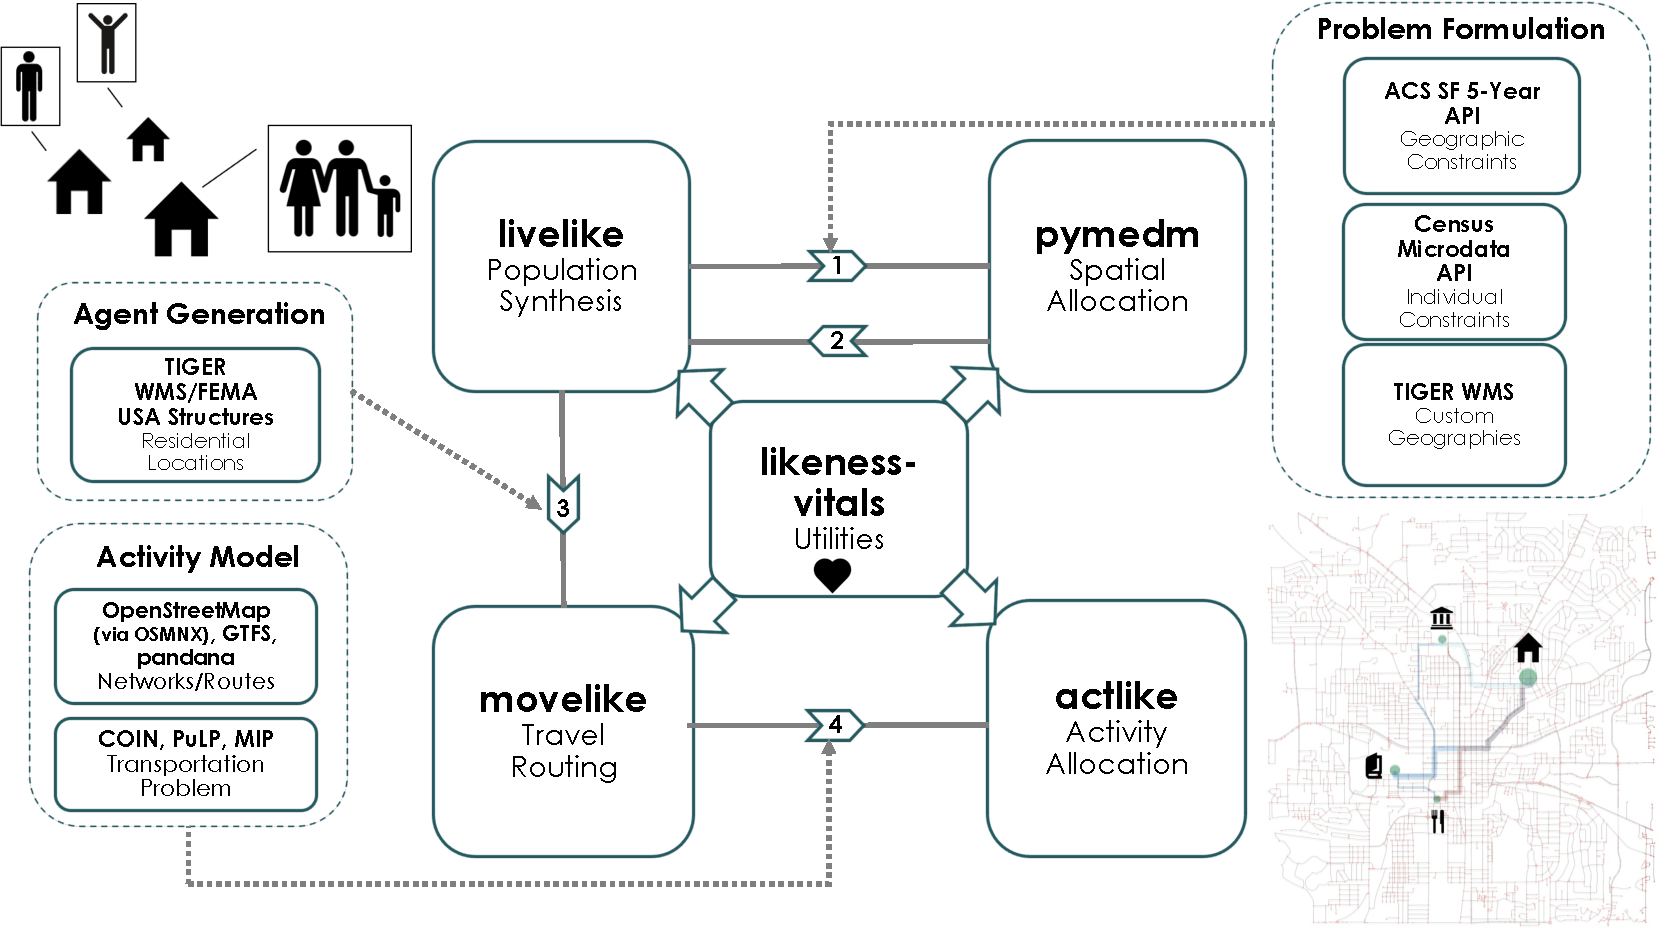
\includegraphics[width=150mm]{figures/ecosystem.pdf}
\caption{Likeness ecosystem overview.}
\label{fig:ecosystem}
\end{figure*}


Synchronous with creating foundational examples for Likeness, we have developed an integrated workflow that scales the ecosystem (\autoref{fig:ecosystem}) to support microsimulation for any metropolitan statistical area (MSA) in the United States.

\autoref{fig:parse-to-attribution} outlines the procedure for agent generation at the MSA level. As discussed in \cite{likeness-scipy-paper-2022}, the \texttt{livelike.acs.puma} class is the core object for residential population synthesis. It stores all census microdata and geographic (e.g., block group, tract) model constraints to support spatial allocation for a single Public-Use Microdata Area (PUMA) in the United States. Residential synthetic populations for MSAs are generated as collections of PUMAs, which are parsed automatically by combining U.S. Census metropolitan/micropolitan delineation files\footnote{https://www.census.gov/geographies/reference-files/time-series/demo/metro-micro/delineation-files.html} with the Census 2010 PUMA-to-tract relationship file\footnote{https://www.census.gov/programs-surveys/geography/technical-documentation/records-layout/2010-tract-to-puma-record-layout.html}. PUMAs parsed for the target MSA are converted into \texttt{livelike.acs.puma} objects in bulk via \texttt{livelike.multi.make\_pumas()}. This function accepts the PUMA Federal Information Processing Standards (FIPS) codes (unique IDs) in list form, along with the target ACS year. This information is then used to gather the relevant ACS Summary File (SF) constraints for spatial allocation of PUMS responses to small census areas of roughly 8,000 people or less (block groups, tracts). Spatial allocation is subsequently handled with parallel processing, which is supported by both packages Likeness offers for Penalized Maximum-Entropy Dasymetric Modeling (P-MEDM) \cite{nagle2014dasymetric}: \texttt{pymedm} (bleeding-edge, Python-native version, based on \texttt{jaxopt} \cite{jaxopt_implicit_diff}) and \texttt{pmedm\_legacy} (stable bridge to original R/C++ routine\footnote{https://bitbucket.org/nnnagle/pmedmrcpp} via \texttt{rpy2}). As demonstrated in \cite{likeness-scipy-paper-2022} and \cite{likeness-scipy-poster-2022}, the population synthesis routine also collects diagnostics on how effectively each P-MEDM solution reproduces variable estimates from the ACS SF relative to reported Margins of Error (MOEs). These utilities are available in both \texttt{pymedm} and \texttt{pmedm\_legacy}.

Likeness generates agents for microsimulation in a way that provides realistic home (origin) locations from which to allocate essential activities on transportation networks. Our initial approach, based on census block-level housing density \cite{likeness-scipy-paper-2022, likeness-scipy-poster-2022}, is now implemented in \texttt{livelike} as a housing universe generation procedure. Additionally, we are actively developing a method (demonstrated in \nameref{section:LCFL}) that enhances this capability by matching synthesized households to residential locations from building footprint data.  These matches are performed by conflating attributes of synthetic households (e.g., dwelling type, income) with building footprint attributes (e.g., floor area, number of units). These utilities are designed to be agnostic to the building footprint provider and can even support
custom building features.

\begin{figure*}[htbp]
\centering
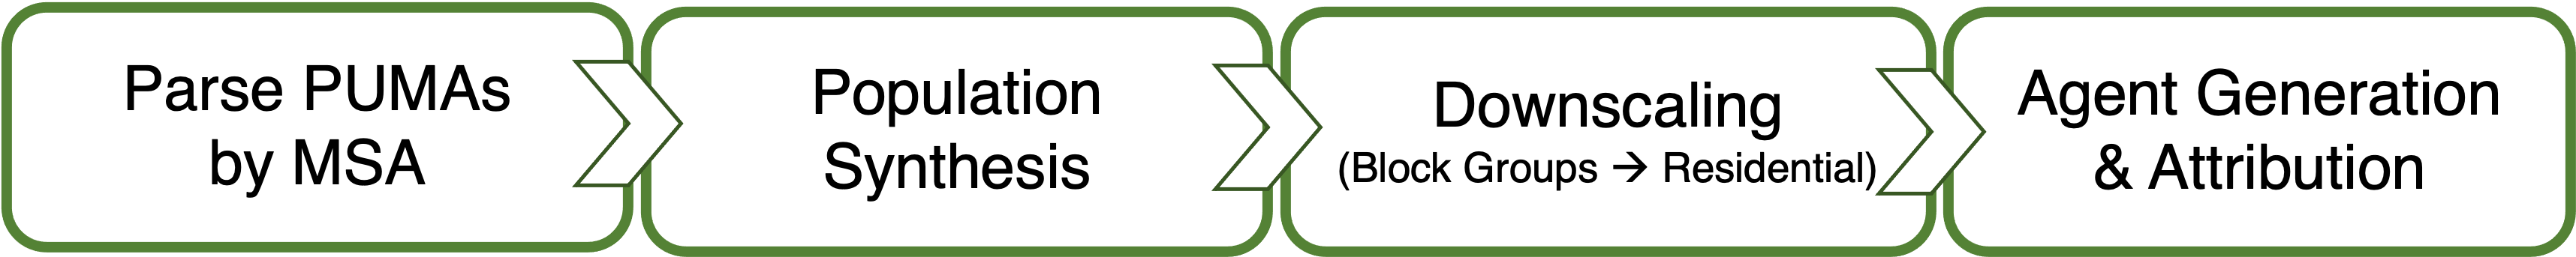
\includegraphics[width=150mm]{figures/parse-to-attribution.png}
\caption{Likeness agent generation procedure for Metropolitan Statistical Areas (MSAs) in the United States.}
\label{fig:parse-to-attribution}
\end{figure*}


Agent residential locations provided by \texttt{livelike} act as origin points for simulating travel to essential activities.
The next stage in the Likeness workflow employs network analysis to model the cost of travel to these activities \cite{OpenStreetMap, osmnx_CEUS_2017, foti_generalized_2012} and allocate agents to POIs accordingly based on mathematical programming routines \cite{mitchell_pulp_2011, santos_mixed_2020, lougee_coin_2003, forrest_coinorcbc_2023}\footnote{The PuLP and Python-MIP open-source optimization Python packages are cited here, along with COIN-OR (a consortium that supports various open-source Operations Research projects) and the COIN-OR Branch-and-Cut solver.}. In our first iteration of Likeness, both these tasks were accomplished within \texttt{actlike}. However, we concluded that the network modeling piece was specialized enough to be split from the \texttt{actlike} package, which led to the creation of \texttt{movelike}. With a push for varied modes of network traversal, three new modes of travel can now be modeled: walking, biking, and public transit. However, modeling travel behavior via public transportation is less straightforward than for driving, biking, and walking networks due to stricter network topology, including factors like connectivity and directionality of routes. We have made our foray into modeling more realistic public transit behavior within \texttt{movelike} through the incorporation of the General Transit Feed Specification (GTFS)\footnote{https://gtfs.org/}. GTFS is a data specification that stipulates the required files, along with their structure and format\footnote{https://gtfs.org/schedule/reference/\#dataset-files}, for publishing, ingesting, and utilizing public transit datasets. The GTFS datasets can be obtained via services such as \textit{TransitFeeds}\footnote{https://transitfeeds.com/} and \textit{The Mobility Database Catalogs}\footnote{https://github.com/MobilityData/mobility-database-catalogs}. In our current iteration we utilize GTFS data feeds to implement a pseudo-transit network space by which agents can engage in limited traversal. This is accomplished through a mask of \textit{OpenStreetMap}\footnote{https://www.openstreetmap.org/} (OSM) street segments known to be associated with bus routes. The OSM network is masked by passing a (multi)polygon feature of buffered and unioned bus routes within the study area into \texttt{osmnx} \cite{osmnx_CEUS_2017}. This method demonstrates progression in representing public transit but certainly has room for improvement, which will be discussed in \nameref{section:dev-roadmap}.

Finally -- and at the heart of it all -- expansion and scaling of the Likeness ecosystem led to the development of a new package for common utilities, \texttt{likeness-vitals}. The \texttt{likeness-vitals} package provides support for monitoring and timing processes, data manipulation, shared spatial functionality, and Census API access.

\subsection{Integrated Demonstration: Leon County, Florida} \label{section:LCFL}

Following the workflow described in Section~\nameref{section:likeness-expansion-scaling}, we demonstrate the current capabilities of Likeness and validate our activity allocation routine for Leon County, Florida. Leon County, whose primary city is Tallahassee, features a population of just under 300,000 residents, a compact urban footprint, and a diverse array of transportation modes (driving, transit, bike, walking). Our mobility validation exercise is based on grocery store visits from simulated home locations. Grocery stores provide a useful test case, acting both as catchments for the general population as well as points of access to vital services including food and healthcare. We obtained grocery store visits from Foursquare's Research Visits feed, which provides POI visitation data attributed by demographic cohort (gender by age) for a variety of facility types\footnote{https://location.foursquare.com/places/docs/how-does-places-work}\textsuperscript{,}\footnote{https://location.foursquare.com/visits/docs/research-feed-schema}.

We first simulated a single synthetic population for the Tallahassee Core-Based Statistical Area (CBSA). Spatial allocation (P-MEDM) was constrained on variables across subjects including sampling universe totals (i.e., population, housing units, households), descriptive factors including demographics, socioeconomic status, housing, mobility, and worker and student characteristics. For the remainder of the analysis, we focused on Leon County alone, removing large outlying areas of the MSA (PUMA \texttt{1206300}, ``Apalachee Region (Outside Leon County)''). Agents\footnote{Agents less than 20 years old were not included in the Foursquare POI data, thus they are excluded from our analysis.} were generated with the Federal Emergency Management Agency's (FEMA) open USA Structures database \cite{yang2018building, usa_struct_2022}. Our allocation procedure leveraged \texttt{livelike} utilities to match synthetic households to single-family residential, multi-family residential, mobile homes, and group quarters housing types.

We used employment and travel mode characteristics to assign agents to transportation networks used to access grocery POIs from home locations. Agents labeled as `employed' possess an associated flag that identifies reported commute mode that can take the following values: `car\_truck\_van', `bicycle', `walked', `wfh', `public\_transportation', `other', and `motorcycle'. Because detailed travel modes are unavailable for agents that are not employed (e.g., retired, active military), we rely on private (i.e., household-level) vehicle ownership instead.

\begin{figure*}[htbp]
\centering
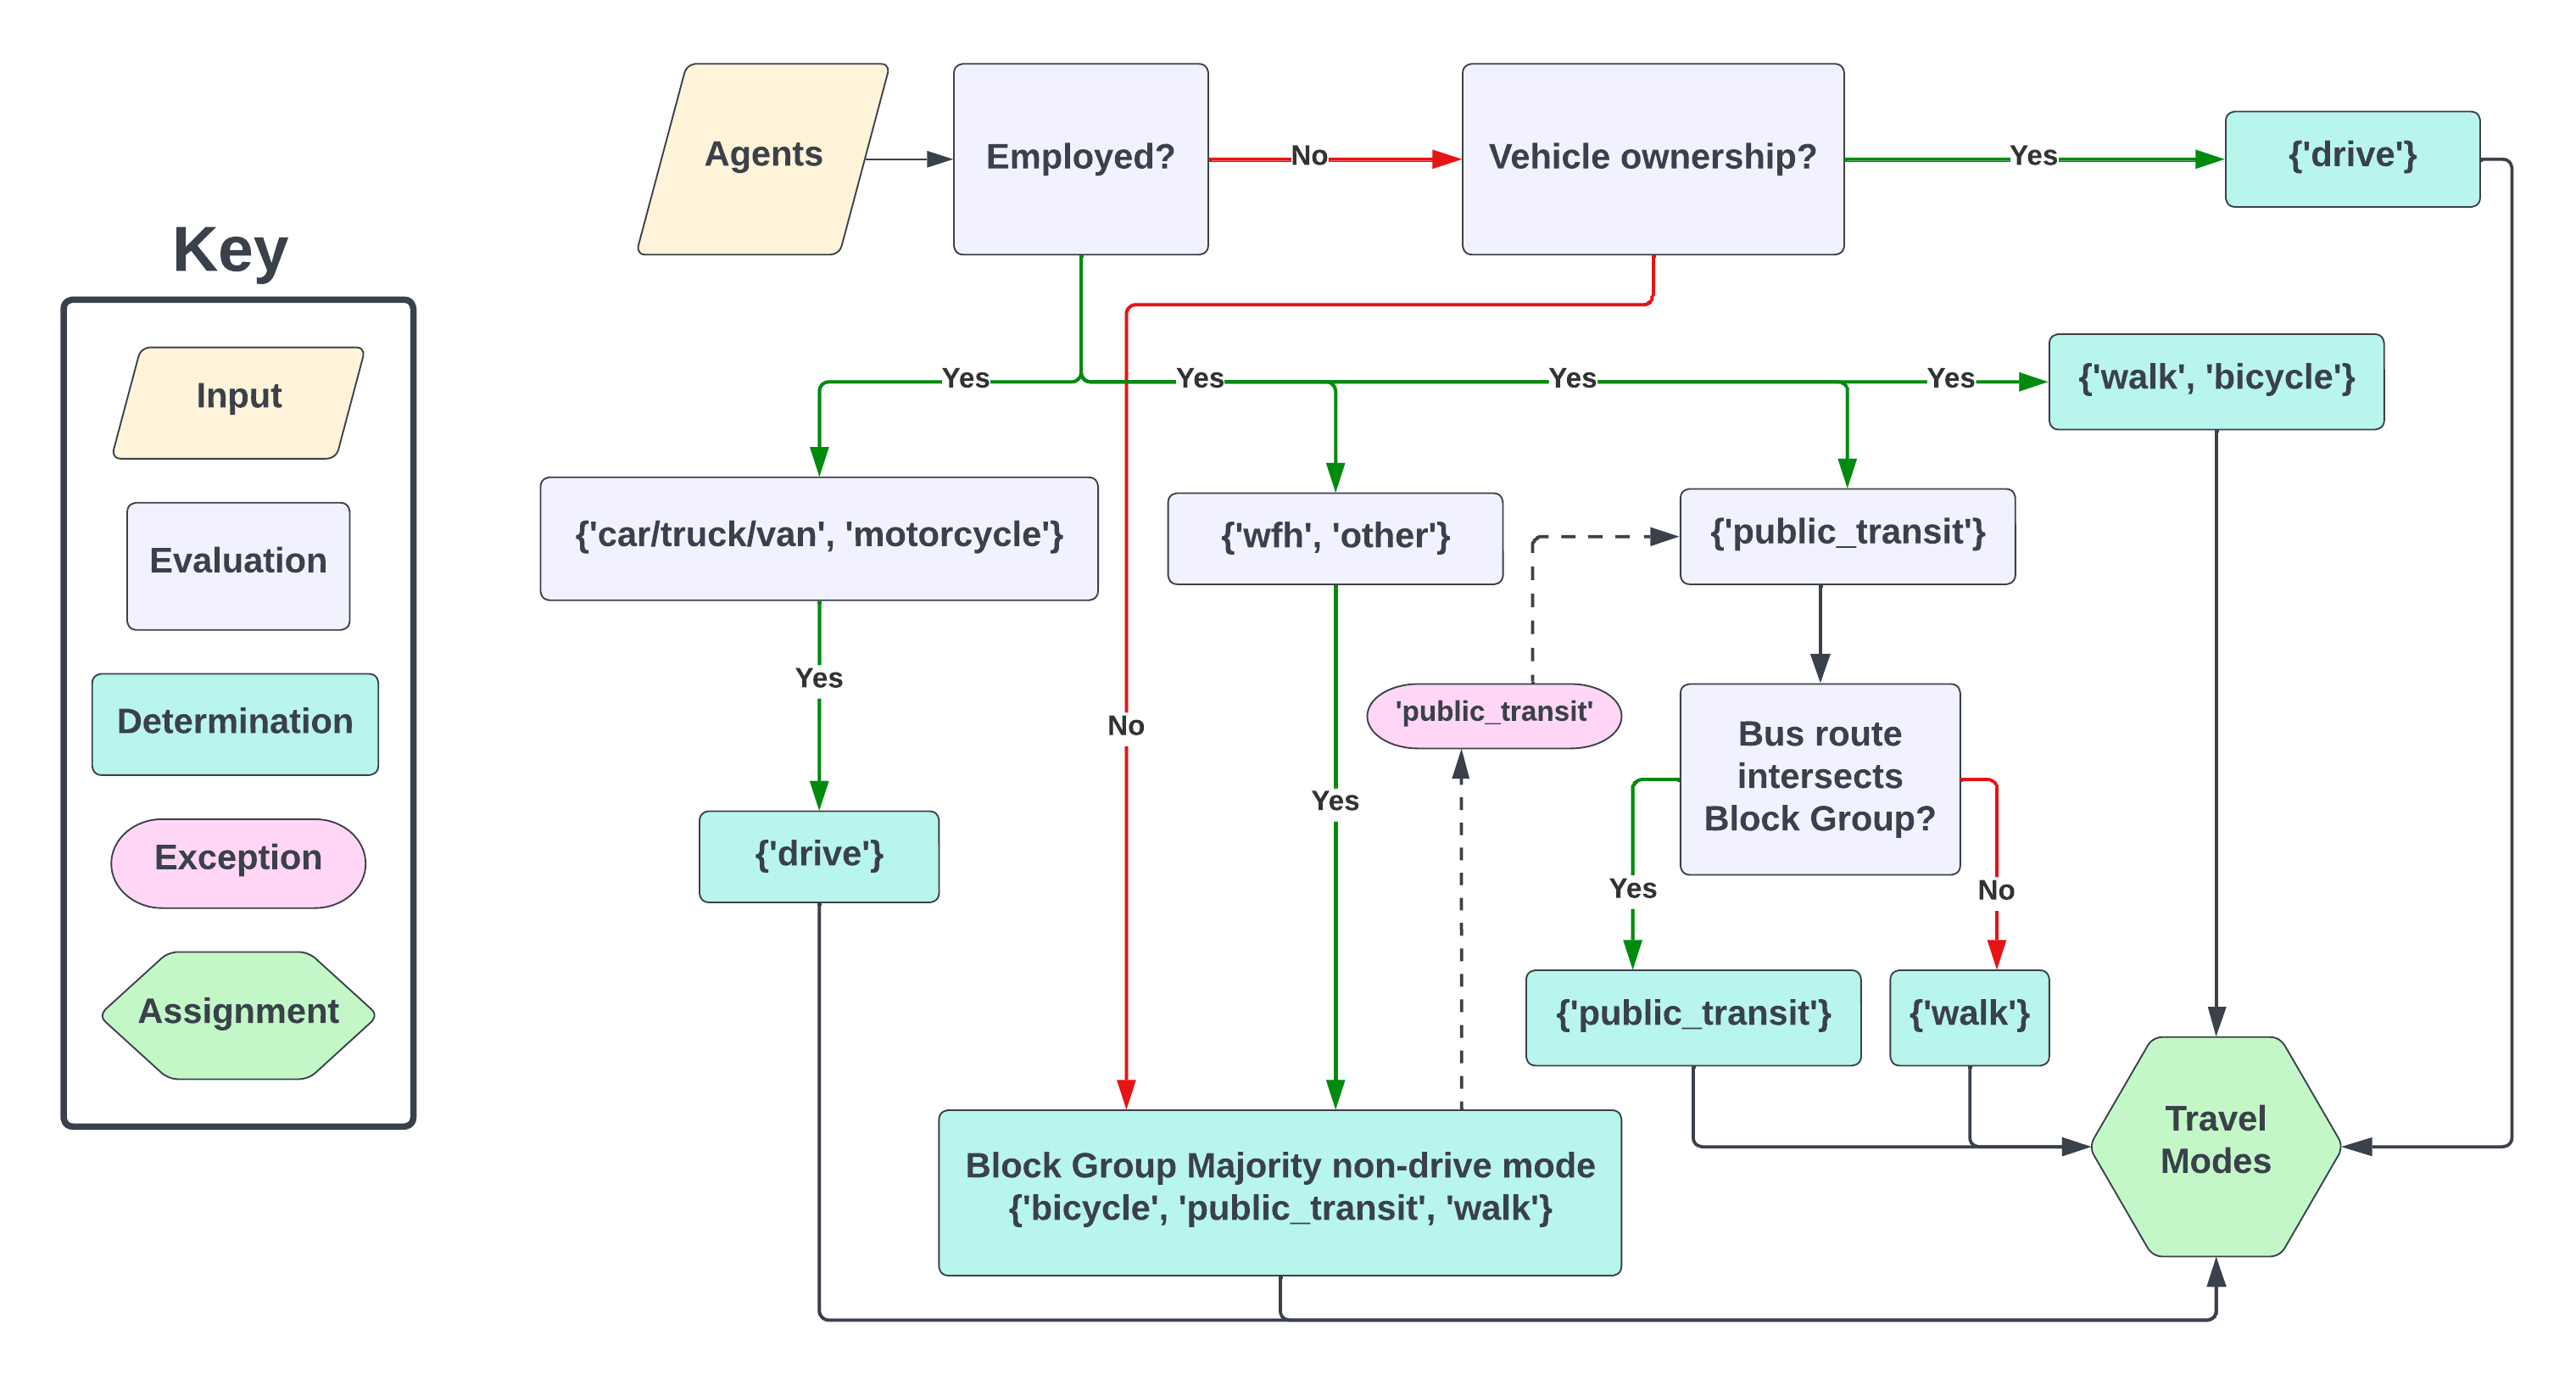
\includegraphics[width=150mm]{figures/mode_assign_workflow.png}
\caption{Agent travel mode assignment decision tree.}
\label{fig:mode_assign_workflow}
\end{figure*}


Travel modes assigned to each agent were conflated with four transportation network types: `walked', `bicycle', `public\_transportation', and `drive'. We supported this process by developing a decision tree, visualized in \autoref{fig:mode_assign_workflow}, through which we assume:

\begin{itemize}
    \item Employed agents will use the transportation network that best matches their commute mode to access grocery POIs.
    \item Agents that are not employed will use a privately-owned vehicle, and thus the `drive' network, to access grocery POIs when available.
    \item Agents that are not employed and lack a privately-owned vehicle will use public transportation if they are located in a block group that is served by Tallahassee's bus network (StarMetro) and opt to walk otherwise.
\end{itemize}

As demonstrated in \autoref{tab:agents_counts_travel_mode}, the `drive' network supports the overwhelming majority of travel to grocery POIs in Leon County, followed by walking, public transportation, and bicycle access.

\begin{table}[htb]
\caption{Householder agents >20yo per assigned travel mode}
\label{tab:agents_counts_travel_mode}
\small
\vspace{-6pt}
\begin{center}
\begin{tabular}{lr}
\toprule
\bf Mode Assignment & \bf Agent Count\\
\midrule
\texttt{'walked'}                   &       5,325       \\
\texttt{'bicycle'}                  &       1,052     \\
\texttt{'public\_transportation'}   &       3,830     \\
\texttt{'drive'}                    &     101,681      \\
\cline{2-2}
                                    &     111,888   \\
\bottomrule
\end{tabular}
\end{center}
\end{table}

\autoref{fig:2x2_agents_hex} shows that Leon County's agent population is distributed unevenly relative to assigned travel modes. Because Leon County's infrastructure primarily supports travel by car, agents who drive are distributed closest to the area's general population density. The spatial distribution of agents who travel by walking also tends to follow Leon County's settlement patterns, though in more limited numbers than for those who drive. Agents using public transport, meanwhile, are largely present in and near the center of the county, roughy occupying denser urban areas where StarMetro service is available. Bicyclists are distributed similarly to bus takers, but with several individual clusters associated with smaller outlying towns and settlements.

\begin{figure}[htbp]
\centering
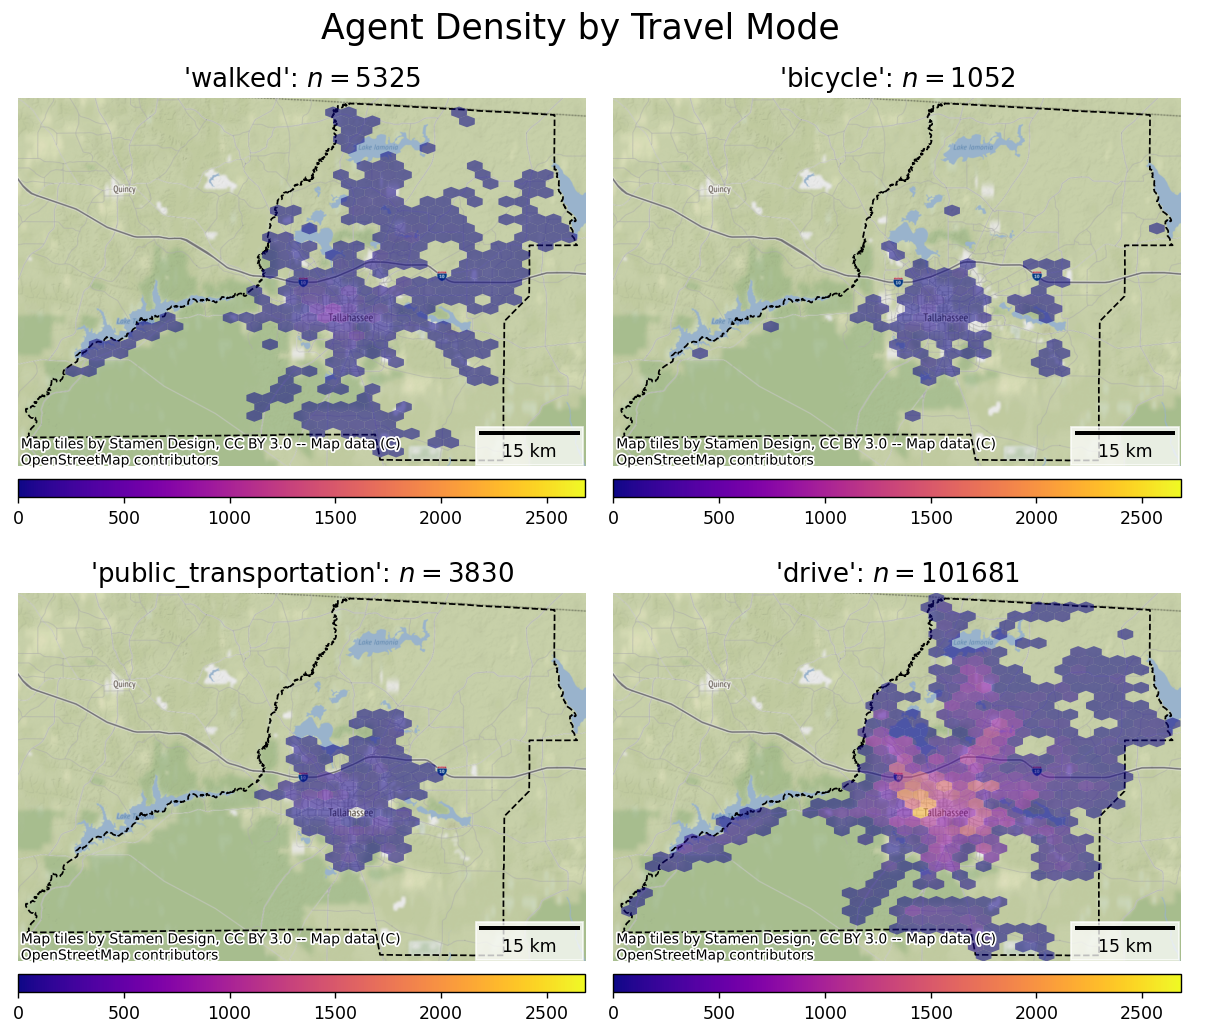
\includegraphics[width=85mm]{figures/2x2_agents_hex.png}
\caption{Synthetic population distribution by travel mode.}
\label{fig:2x2_agents_hex}
\end{figure}


Grocery store POIs with medium to high visit confidence (at least 30 device visits per month, $n$ = 53) were obtained from Foursquare for Leon County in January 2023. Destination capacities were estimated based on visit counts weighted by representativeness of the demographic cohort within the state's 2010 Census population\footnote{https://location.foursquare.com/visits/docs/foursquare-data-normalization}. Destination capacities were estimated by the daily average (mean) for each POI during the collection month (01/2023).

After travel modes were assigned to agents, four network cost matrices were calculated from origin (residential location) to destination (grocery store) POIs in \texttt{movelike}. Agents were then allocated to a single probable destination POI based on least cost network travel paths with the \texttt{actlike.ActivityAllocation} routine, which solves a modified Transportation Problem\footnote{This model is formulated in \cite{likeness-scipy-paper-2022}.} \cite{hitchcock_distribution_1941, koopmans_optimum_1949, miller_geographic_2001, tp_miller_gc__2015}, where destination POI capacities are scaled \cite{lovelace_truncate_2013} by the proportion of assigned travel mode for each scenario. All models were run consecutively on two machines for benchmarking purposes. These were:

\begin{itemize}
    \item A personal laptop (macOS) with a 2.3 GHz Quad-core Intel Core i7 processor (32 GB RAM).
    \item A virtual machine (Ubuntu) with a 2.8 GHz 22-core Intel(R) Xeon(R) processor (86 GB RAM).
\end{itemize}

The large disparity in problem size seen in \autoref{tab:agents_counts_travel_mode} is even more pronounced in solution runtimes, shown in \autoref{tab:allocation_solution_runtime}. Optimal solutions for non-drive models were found in a maximum time of just over 1 minute on both machines, with the drive model taking more than 17 and 8 hours to solve on the macOS and Ubuntu machines, respectively. Considering the solution time for the drive scenario, there is clearly a need for a more effective solution technique, which will be further discussed in \nameref{section:dev-roadmap}.

\begin{table}[htb]
\caption{Allocation Solution Runtimes (min.)}
\label{tab:allocation_solution_runtime}
\small
\vspace{-6pt}
\begin{center}
\begin{tabular}{lrr}
\toprule
\bf Mode Assignment & \bf macOS     & \bf Ubuntu \\
                    & 4 cores       & 22 cores \\
                    & 32 GB RAM     & 86 GB RAM \\
\midrule
\texttt{'walked'}                   &       0.72    &   1.19    \\
\texttt{'bicycle'}                  &       0.05    &   0.26    \\
\texttt{'public\_transportation'}   &       0.48    &   0.69    \\
\texttt{'drive'}                    &    1061.43    & 483.94    \\
\bottomrule
\end{tabular}
\end{center}
\end{table}

\subsubsection{Validation procedures}

Our validation procedures were designed to quantify the degree to which Likeness 1) resembles reference population estimates provided by the ACS SF with the synthetic populations (\textbf{demographic validation}) and 2) allocates activities matching real-world visitation patterns by demographics segments captured by the Foursquare POI data (\textbf{mobility validation}).

To produce our demographic validation, we followed \cite{urbanpop-AG-2023} and measured our synthetic populations' degrees of conformity with 90\% Margins of Error (MOEs) available from the ACS SF. ACS MOEs provide bounds for the expected ranges of values that our variables of interest could take. Tabulating individual attributes within each block group's synthetic population results in a reconstruction of the ACS SF estimates that can be assessed against the 90\% MOEs. Greater conformity with the MOEs (``MOE Fit Rate'') indicates a synthetic population that could plausibly resemble that block group's ``true'' population.

Following \cite{urbanpop-AG-2023} and \cite{likeness-scipy-paper-2022}, we ran our mobility validation using Canonical Correlation Analysis (CCA). CCA, which measures the degree of linear association between two multidimensional datasets \cite{hardoon2004canonical}, is necessary to compare visitation patterns ($n$ grocery store locations by $m$ demographic cohorts). We performed CCA on both the between-destination (relative prevalence) and within-destination (compositional) characteristics of each POI by demographic group. Both CCA runs were generated from tabulated counts of trips from the observed and synthetic datasets, their key difference being the method of standardization (column-wise for between-destination, row-wise for within-destination). We used the CCA coefficient of determination ($R^2$) to measure associations between synthetic and observed results. To better understand POI-specific activity allocation performance, we generated an additional local measure of within-destination correspondence. The local within-destination statistic compares the relative sizes of demographic cohorts using Spearman Rank Correlation, a non-parametric measure of the association between the ranks of two variables \cite{zar1972significance}. We opted for Spearman Correlation due to the relatively small number of demographic cohorts ($n$ = 11).

\subsection{Results}\label{section:results}

\subsubsection{Demographic Validation}

\begin{table}[htb]
\caption{Demographic validation}
\label{tab:demographic-validation}
\small
\vspace{-6pt}
\begin{center}
\begin{tabular}{l | p{3.25cm} | c}
\toprule
\bf PUMA & \bf Name & \bf ACS 90\% MOE Fit Rate\\
\midrule
1206300 & Leon County (Central) & 0.992 \\
1207300 & Leon County (Outer) &  0.998 \\
1207301 & Apalachee Region (Outside Leon County) & 0.994 \\
\bottomrule
\end{tabular}
\end{center}
\end{table}

\begin{figure}[htbp]
\centering
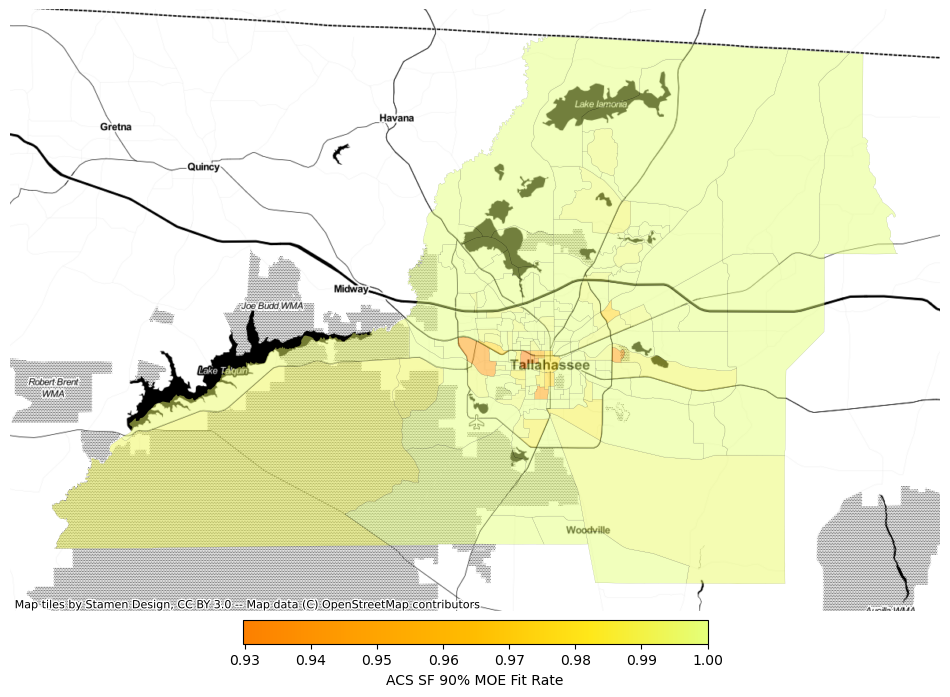
\includegraphics[width=85mm]{figures/local_demographic_validation.png}
\caption{Local demographic validation for Leon County.}
\label{fig:local-demographic-validation}
\end{figure}


Each of the three P-MEDM runs (one for each PUMA in the Tallahassee CBSA) resulted in a synthetic reconstruction of the ACS 90\% MOEs. Overall, these reconstructions matched with at least 99\% of the published MOEs from the ACS SF (\autoref{tab:demographic-validation}. At the more granular level of Leon County block groups (\autoref{fig:local-demographic-validation}), MOE Fit Rates were relatively lower but still in agreement with at least 90\% of the ACS SF MOEs in each location. We observed diminished performance in areas with large group quarters populations (e.g., college dormitories, prisons), as well as more sparsely populated rural and peri-urban portions of Leon County.

\subsubsection{Mobility Validation}

Our mobility simulation more faithfully recreated between-destination demographics ($R^2$ = 0.74) than within-destination demographics ($R^2$ = 0.41) (\autoref{tab:demographic-validation}). Inspecting the local within-destination scores, mapped in \autoref{fig:local-win-cca}, we observed generally greater correspondence between synthetic and observed POI demographics near Tallahassee's downtown core, Florida State University, and Florida A\&M University, with diminished performance in suburban and outlying areas of Leon County.

\begin{figure}[htbp]
\centering
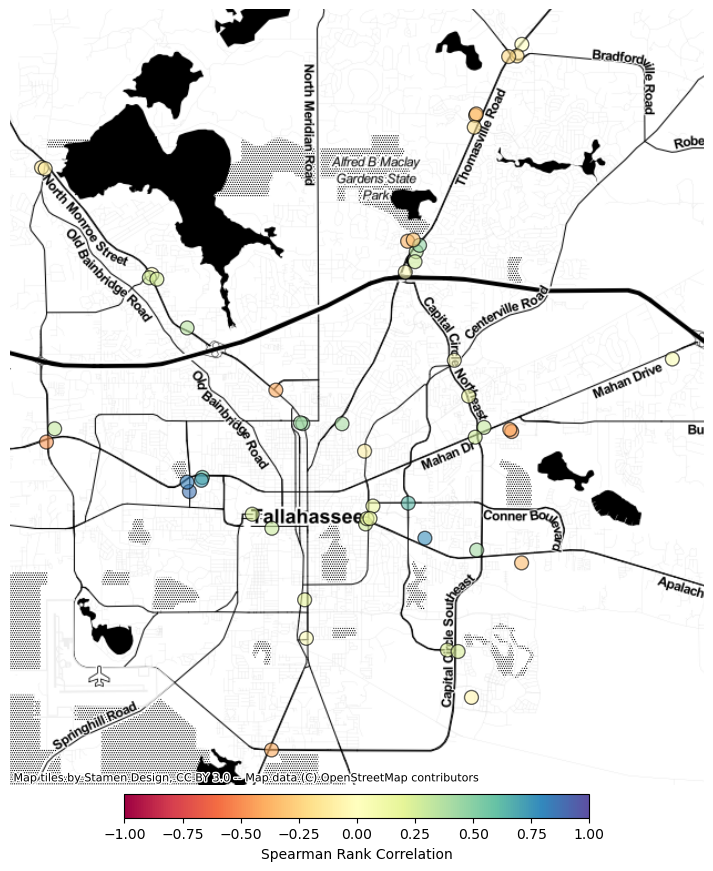
\includegraphics[width=85mm]{figures/local_win_cca.png}
\caption{Local within-POI mobility validation.}
\label{fig:local-win-cca}
\end{figure}


It is difficult to pinpoint the inconsistency in recreating POIs' visitation patterns. In addition to urban density, this is potentially related to diversity of travel modes near the urban core (the increased biking, walking, and public transit use presented in \autoref{fig:2x2_agents_hex}), but it requires further investigation. Section~\nameref{section:limitations} provides some additional confounding factors that are worthy of exploring relative to these results.

\subsection{Limitations}\label{section:limitations}

We found that overall, Likeness approximates travel to non-anchor (grocery store) POIs modestly well. However, its performance tends to be weaker relative to travel to anchor activities (work/school), demonstrated in \cite{likeness-scipy-paper-2022}. This suggests that approximating destination capacities for activities like grocery store visits provide an added challenge for activity allocation, including when real-world observations from visitation data are used. Additionally, multiple confounding factors related to data inputs and model assumptions may have affected our results:

\begin{itemize}
    \item \textbf{Data-Specific:} Our clearest challenge is temporal mismatch between the synthetic population (2019) and POI visit data (2023). We have yet to increment our ACS year due to issues of non-conforming geography between the 2010 PUMAs and 2020 block groups/tracts. We hope to explore solutions to this problem starting with the forthcoming 2022 ACS releases, which will adopt 2020 PUMAs across all geographic levels\footnote{https://www.census.gov/programs-surveys/acs/news/data-releases/2022/release.html}. We were also limited to only one month of POI visit data. In future work, we hope to leverage a longer period of record to account for POIs with consistently high rates of visitation.
    \item \textbf{Model-Specific:} Several large assumptions were made that could confound our results, particularly that 1) agents simultaneously travel to grocery stores, 2) agents only select one grocery store to visit, using only one mode of travel, and 3) travel to grocery stores only occurs between home and work. These assumptions can be updated by incorporating information from time-use and travel surveys into Likeness. In this way, we can better reflect the times of day that different demographic cohorts access various activities \cite{macal2018chisim}.
\end{itemize}

We also hope to tighten our assumptions about the feasibility of POI access relative to the various travel modes. For example, in our current assignment process (\autoref{fig:mode_assign_workflow}) agents unmatchable to a defined travel mode were considered walkers as a fallback for unavailability of a reachable bus route. Future iterations will refine this decision process by considering a distance threshold for agents to be labeled as either walkers or transit users. For example, we could set a rule that walking agents must be located within a reasonable distance of the closest POI, while agents that use bus service should reside near a bus stop in addition to being close to a bus route. To ensure all agents have at least one feasible POI destination to access, we also plan to incorporate a greater variety of curated locations from ORNL's PlanetSense database \cite{thakur2015planetsense}.

\subsection{Conclusion and Outlook}\label{section:conclusion-outlook}

This paper presented enhancements and scaling approaches for the Likeness spatial microsimulation toolkit. These include batched population synthesis runs for MSAs in the United States, residential allocation, and large-scale transportation network generation. We demonstrated these new capabilities by developing a mobility validation exercise for Leon County, FL. Our results provided reasonable representation of neighborhood demographics and routing to nearby essential services (grocery stores), with more mixed results related to activity allocation. The activity allocation results, however, do provide new research directions that we plan to explore in our future work. These include temporality of POI travel (travel probabilities relative to demographic cohorts), behavioral factors (willingness to travel given cost and impedances), and the use of multiple travel modes to reach activities.

Given the relative success of our population synthesis procedures in Section~\nameref{section:LCFL}, we are interested in also applying Likeness to explore transportation equity in the context of access to essential services like food and healthcare. Such an approach would aim to enhance existing research on transportation and accessibility \cite{horner_2015, wood_2016} with a cross-sectional representation of social, demographic, housing, and mobility characteristics. Assuming an agent with some blend of socio-demographic and economic characteristics resides in a particular section of a neighborhood, how many essential services can be readily accessed using their assigned transportation network? Using the Likeness ecosystem, we could develop such a measure for all agents in a synthetic population, allowing the comparison of accessibility to population metrics like mobility difficulty. These insights could in turn be used to guide urban/regional infrastructure planning, pinpointing areas where drive, transit, or bike/walk services could be improved or expanded.

\subsection{Development Roadmap: 2023 - 2024} \label{section:dev-roadmap}

\begin{itemize}
    \item \textbf{Tooling for custom geographic extents.} The MSA-specific workflow demonstrated in this paper is limited in that it does not support custom geographic extents. This prevents analysis, for example, of predominantly rural areas.
    We are actively developing an approach to create residential synthetic populations for custom areas of interest (AOIs), supported by USA Structures. This functionality will also support the development of synthetic populations with national-scale coverage.
    \item \textbf{Open-sourcing core packages.} Though we have yet to meet our goal of open-sourcing the suite of Likeness packages \cite{likeness-scipy-paper-2022}, we are still on track to release the core packages for residential population synthesis, \texttt{pymedm} and \texttt{livelike}, in 2023. Releases of \texttt{movelike} and \texttt{actlike} are likely to follow in 2024.
    \item \textbf{Packaging schema.} A further consideration related to open-sourcing is whether we should migrate from a confederated toolkit schema where each module is a semi-independent Python package, as is seen in the modern implementation of PySAL \cite{pysal_GA_2022}, to a single monolithic Python package with submodules. Each schema has benefits, and this decision will require much consideration. With regards to the current confederated schema, the main benefit is modularity and reduced burden for continuous integration testing runtimes. This primary benefit is from a developer standpoint. However, providing a single package to install and use is a clear benefit to the user.
    \item \textbf{Consolidating visualization functionality.} We are in the process of consolidating functionality related to the visualization of input, processing, and results that have been used in an ad-hoc manner in the past. An initial push will be made for the inclusion of ``made-to-order'' population density hexbin plots and network-space allocation routes.
    \item \textbf{Improving mobility modeling.} Modeling public transit is a key area where we intend to develop increasingly more realistic agent ``choices.'' As stated previously in \nameref{section:likeness-expansion-scaling}, there is significant potential in exploring further integration of GTFS data for locally-accurate modeling.
    \item \textbf{Optimization bottleneck.} As demonstrated in \nameref{section:results}, there is a clear hit in computational performance and runtime when solving  \texttt{actlike.ActivityAllocation} problems on increasingly larger model instances (e.g., more agents and more POIs). There are two paths to resolving this issue (which may be considered in concert): 1) Reviewing our modified Transportation Problem mixed-integer program (formulated in \cite{likeness-scipy-paper-2022}); and 2) Utilizing a new underlying solver engine, such as HiGHS\footnote{https://highs.dev/} \cite{highs_mpc_2018}.
    In reviewing our formulation we will first investigate the potential for generating fewer constraints in the model. Following this, as stated above, we may consider formulating the model in a new solver. Depending on the outcome of these experiments we may consider a new underlying optimization problem or implement a heuristic.
\end{itemize}

\subsection{Acknowledgements}

The authors would like to thank Ty Frazier for his contributions to scoping the incorporation of General Transit Feed Specification (GTFS) data during an earlier phase of this project.

The authors would also like to thank the two volunteer reviewers for their constructive feedback and the SciPy Proceedings editorial team for their ongoing support.

Notice: Research reported in this publication was supported by the National Center For Advancing Translational Sciences of the National Institutes of Health under Award Number UL1-TR001409, KL2-TR001432 \& TL1-TR001431. The content is solely the responsibility of the authors and does not necessarily represent the official views of the National Institutes of Health.

This manuscript has been authored by UT-Battelle, LLC under Contract No. DE-AC05-00OR22725 with the U.S. Department of Energy. The United States Government retains and the publisher, by accepting the article for publication, acknowledges that the United States Government retains a non-exclusive, paid-up, irrevocable, world-wide license to publish or reproduce the published form of this manuscript, or allow others to do so, for United States Government purposes. The Department of Energy will provide public access to these results of federally sponsored research in accordance with the DOE Public Access Plan (http://energy.gov/downloads/doe-publicaccess-plan).

